\chapter{Espectroscopia eletrônica e fotofísica}\label{ch:b3:electronic-spectroscopy}

Sob a lâmpada ultravioleta de um bar escuro, um copo de água tônica brilha
com um azul pálido, fantasmagórico. O quinino que ela contém absorve a luz
ultravioleta, que o olho não vê, e devolve parte dela alguns nanossegundos
depois como luz azul visível. Absorção, uma vida curta em um estado excitado,
emissão em um comprimento de onda maior, a energia que não volta como luz: o
destino de uma molécula excitada é uma competição entre processos com
constantes de velocidade, e seu espectro é moldado pelas vibrações da
molécula e pelas regras de simetria do \cref{ch:b3:group-theory-applied}. Este
capítulo estuda as transições eletrônicas e o que acontece depois delas, o
assunto chamado fotofísica; o \cref{ch:b3:photochemistry} acrescenta os casos
em que a molécula excitada reage.

\begin{recall}
O volume do 1.º ano mediu a absorbância com a lei de Beer--Lambert, $A =
\varepsilon\ell c$, definiu o coeficiente de absorção molar, os cromóforos e os
sistemas conjugados, e relacionou a cor ao máximo de absorção. O volume do
2.º ano designou os orbitais de fronteira HOMO e LUMO. O \cref{ch:b3:many-electron-atoms}
definiu os \omterm{def:b3:many-electron-atoms:singlet-triplet}{estados singleto} e tripleto; o \cref{ch:b3:group-theory-applied}, o
teorema das integrais nulas; o \cref{ch:b3:rovibrational-spectroscopy}, os
níveis vibracionais de uma ligação.
\end{recall}

\begin{omfigure}
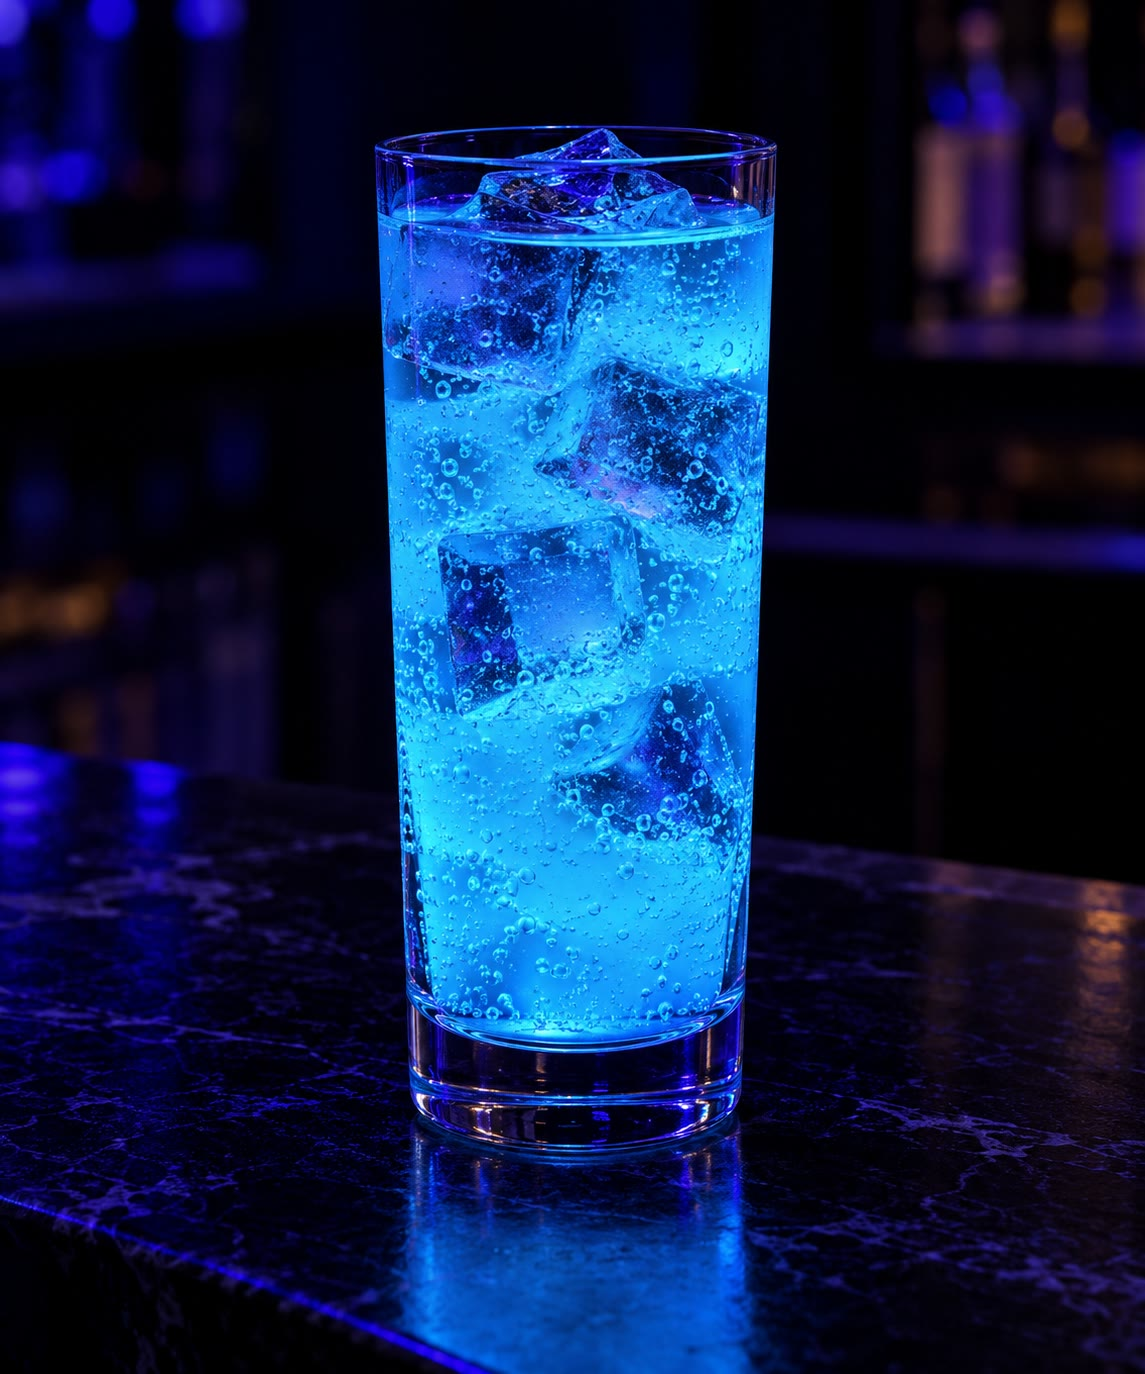
\includegraphics[height=4.6cm]{images/book4/ai/b3-07-tonic.jpg}\hspace{1em}%
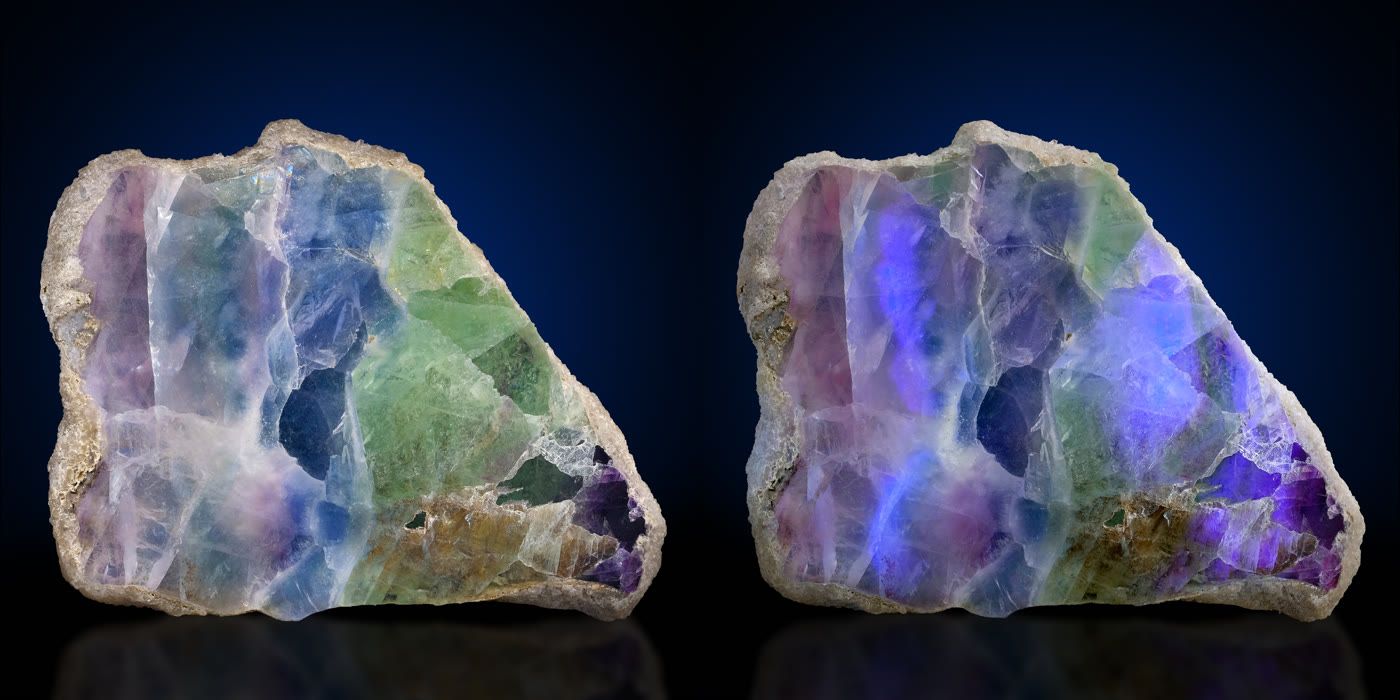
\includegraphics[height=4.6cm]{images/book4/fluorite-uv.jpg}

{\small À esquerda: água tônica brilhando em azul sob uma lâmpada ultravioleta.
À direita: fluorita à luz do dia e fluorescendo sob luz ultravioleta; o
mineral deu nome à \omterm{def:b3:electronic-spectroscopy:luminescence}{fluorescência}. Fotografia de Masha Milshina, CC BY 4.0.}
\end{omfigure}

\section{Transições eletrônicas e suas regras de seleção}

\begin{definition}[Momento dipolar de transição, força do oscilador]\label{def:b3:electronic-spectroscopy:transition-dipole}
O \emph{momento dipolar de transição}\index{momento dipolar de transicao@momento dipolar de transição} entre os
estados $\Psi_i$ e $\Psi_f$ é $\boldsymbol\mu_{fi} = \langle\Psi_f|\hat{\boldsymbol\mu}|\Psi_i
\rangle$, com $\hat{\boldsymbol\mu} = -e\sum_k\mathbf r_k$ (mais as cargas
nucleares, que se cancelam entre estados ortogonais). A \emph{força do
oscilador}\index{forca do oscilador@força do oscilador} $f$ é a medida adimensional da
intensidade de uma banda, cerca de 1 para as transições mais intensas.
\end{definition}

\begin{proposition}[Intensidade e força do oscilador]\label{prop:b3:electronic-spectroscopy:intensity}
A absorção integrada de uma banda é proporcional a $|\boldsymbol\mu_{fi}|^2$,
e, na prática,
\[
f \approx 4.32\times10^{-9}\int\varepsilon(\tilde\nu)\,\dd\tilde\nu,
\]
com $\varepsilon$ em \unit{L.mol^{-1}.cm^{-1}} e $\tilde\nu$ em \unit{cm^{-1}}.
\end{proposition}
\admitted

A proporcionalidade vem da teoria de perturbação dependente do tempo, e o
fator numérico, do oscilador clássico; ambos são tratados em cursos mais
avançados. O que importa aqui é que $f$ só é grande quando
$\boldsymbol\mu_{fi}$ o é, e que a simetria pode forçá-lo a zero.

\begin{theorem}[A regra de seleção de spin]\label{thm:b3:electronic-spectroscopy:spin-rule}
Uma transição de dipolo elétrico entre estados de spin total diferente é
proibida: $\Delta S = 0$.
\end{theorem}

\begin{proof}
Cada estado é o produto de uma função espacial por uma função de spin, $\Psi = \phi\,\chi$.
O \omterm{def:b3:quantum-model-systems:operator}{operador} dipolo age apenas sobre as posições, logo $\langle\phi_f\chi_f|\hat{\boldsymbol\mu}|
\phi_i\chi_i\rangle = \langle\phi_f|\hat{\boldsymbol\mu}|\phi_i\rangle\langle\chi_f|\chi_i\rangle$.
Funções de spin de $S$ diferentes são \omterm{def:b3:quantum-model-systems:operator}{autofunções} de $\hat S^2$ com \omterm{def:b3:quantum-model-systems:operator}{autovalores}
diferentes, logo ortogonais (\cref{thm:b3:quantum-model-systems:hermitian-real}):
o segundo fator se anula.
\end{proof}

\begin{theorem}[A regra de Laporte]\label{thm:b3:electronic-spectroscopy:laporte}
Em uma molécula com \omterm{def:b3:point-groups:inversion}{centro de inversão}, uma transição de dipolo elétrico deve
mudar a paridade: $g \leftrightarrow u$ é permitida, $g \leftrightarrow g$ e $u
\leftrightarrow u$ são proibidas. É a \emph{regra de Laporte}\index{regra de Laporte}.
\end{theorem}

\begin{proof}
As componentes de $\hat{\boldsymbol\mu}$ trocam de sinal sob a inversão: são $u$.
O produto $\Gamma_f\otimes\Gamma_\mu\otimes\Gamma_i$ só é $g$ se $\Gamma_f$ e $\Gamma_i$
têm paridades opostas; caso contrário, é $u$ e não pode conter a \omterm{def:b3:group-theory-applied:reducible}{representação
totalmente simétrica} (\cref{thm:b3:group-theory-applied:vanishing-integral}).
\end{proof}

As duas regras são estritas para os estados idealizados; as moléculas reais as
relaxam --- o \omterm{def:b3:many-electron-atoms:spin-orbit}{acoplamento spin--órbita} mistura os caracteres singleto e tripleto,
as vibrações removem o centro de simetria por um instante --- e as transições
``proibidas'' aparecem, fracas. As bandas $d$--$d$ dos complexos octaédricos,
proibidas por Laporte e fracas, devem sua cor a esse relaxamento
(\cref{ch:b3:complex-spectra-magnetism}).

\begin{definition}[Transição de transferência de carga]\label{def:b3:electronic-spectroscopy:charge-transfer}
Uma \emph{transição de transferência de carga}\index{transicao de transferencia de carga@transição de transferência de carga} leva um
elétron de um orbital localizado principalmente em uma parte de um sistema (um
doador) para um orbital localizado principalmente em outra (um aceptor); seu
dipolo de transição é grande, sua banda intensa e larga, e sua energia sensível
à polaridade do solvente.
\end{definition}

\begin{method}[Atribuir uma banda de absorção]\label{met:b3:electronic-spectroscopy:assign-band}
\begin{enumerate}
  \item $\varepsilon_{\max}$ acima de cerca de \qty{e4}{L.mol^{-1}.cm^{-1}}: uma transição
        permitida ($\pi\to\pi^*$ de um sistema conjugado, ou transferência de carga).
  \item $\varepsilon_{\max}$ de 10 a algumas centenas: uma transição proibida ($n\to\pi^*$,
        proibida por simetria; $d$--$d$, proibida por Laporte).
  \item $\varepsilon_{\max}$ abaixo de 1: proibida por spin.
  \item Uma banda $n\to\pi^*$ se desloca para comprimentos de onda menores em
        solventes próticos (o par não ligante é estabilizado por ligações de
        hidrogênio); uma banda $\pi\to\pi^*$, em geral, para maiores.
\end{enumerate}
\end{method}

\section{O princípio de Franck--Condon}

\begin{theorem}[Princípio de Franck--Condon]\label{thm:b3:electronic-spectroscopy:franck-condon}
Na \omterm{def:b3:computational-chemistry:born-oppenheimer}{aproximação de Born--Oppenheimer}, e se o dipolo de transição depende pouco
das posições nucleares, a intensidade da \omterm{def:b3:electronic-spectroscopy:vibronic}{transição vibrônica} do nível
vibracional $v''$ do estado eletrônico inferior ao nível $v'$ do superior é
proporcional a $|\langle\chi_{v'}|\chi_{v''}\rangle|^2$, o quadrado da
sobreposição das duas funções de onda vibracionais: é o \emph{princípio de
Franck--Condon}\index{principio de Franck--Condon@princípio de Franck--Condon}. As
transições eletrônicas são verticais: os núcleos não se movem enquanto os elétrons saltam.
\end{theorem}

\begin{proof}
Com $\Psi = \psi_{\mathrm{el}}(\mathbf r;R)\chi_v(R)$, o momento de transição é
$\int\chi_{v'}^*\big[\int\psi'^*_{\mathrm{el}}\hat\mu\psi''_{\mathrm{el}}\dd\mathbf r\big]
\chi_{v''}\,\dd R$. O colchete é o momento de transição eletrônico
$\mu_{\mathrm{el}}(R)$; tomado como constante (a aproximação de Condon), ele sai da
integral, deixando $\mu_{\mathrm{el}}\langle\chi_{v'}|\chi_{v''}\rangle$.
\end{proof}

\begin{definition}[Transição vibrônica, progressão, fator de Franck--Condon]\label{def:b3:electronic-spectroscopy:vibronic}
Uma \emph{transição vibrônica}\index{transicao vibronica@transição vibrônica} muda ao mesmo
tempo os estados eletrônico e vibracional; as raias $v' \leftarrow 0$ para $v' = 0, 1, 2,
\dots$ formam uma \emph{progressão vibrônica}\index{progressao vibronica@progressão vibrônica}; o
\emph{fator de Franck--Condon}\index{fator de Franck--Condon} de uma raia vibrônica é
$|\langle\chi_{v'}|\chi_{v''}\rangle|^2$.
\end{definition}

\begin{proposition}[Osciladores deslocados]\label{prop:b3:electronic-spectroscopy:displaced}
Se os dois estados são harmônicos com a mesma frequência e o mínimo superior
está deslocado de $\Delta$ (em unidades de $\sqrt{\hbar/m\omega}$), os \omterm{def:b3:electronic-spectroscopy:vibronic}{fatores
de Franck--Condon} a partir de $v'' = 0$ formam uma distribuição de Poisson,
$|\langle v'|0\rangle|^2 = \eu^{-S}S^{v'}/v'!$, com $S = \Delta^2/2$; a raia mais intensa
fica perto de $v' = S$.
\end{proposition}
\admitted

A demonstração geral usa os \omterm{def:b3:quantum-model-systems:ladder}{operadores escada} do
\cref{ch:b3:quantum-model-systems}; os dados das figuras deste capítulo
verificam a fórmula por integração direta. Um deslocamento pequeno dá uma
raia 0--0 intensa; um grande, uma progressão longa cujo membro mais intenso
fica longe da raia 0--0.

\begin{omfigure}
\begin{tikzpicture}
\begin{axis}[name=pc, width=0.46\linewidth, height=6cm, xmin=-4, xmax=5, ymin=0,
  ymax=14, axis lines=left, xtick=\empty, ytick=\empty, xlabel={coordenada nuclear},
  ylabel={energia}, label style={font=\small}]
\addplot[black, thick] table[x=y, y=ground] {figdata/out/bachelor-3-franck-condon-curves.dat};
\addplot[omDef, thick] table[x=y, y=excited] {figdata/out/bachelor-3-franck-condon-curves.dat};
\draw[omabs] (axis cs:0,0.5) -- (axis cs:0,10.6);
\draw[omvib] (axis cs:-1,0.5) -- (axis cs:1,0.5);
\draw[omvib] (axis cs:0.732,9.5) -- (axis cs:2.732,9.5);
\draw[omvib] (axis cs:-0.000,10.5) -- (axis cs:3.464,10.5);
\draw[omvib] (axis cs:-0.504,11.5) -- (axis cs:3.968,11.5);
\draw[omvib] (axis cs:-0.914,12.5) -- (axis cs:4.378,12.5);
\node[font=\small, anchor=west] at (axis cs:-3.9,13.0) {excitado};
\node[font=\small, anchor=west] at (axis cs:3.0,1.5) {fund.};
\node[font=\scriptsize, anchor=east] at (axis cs:-0.05,5.5) {vertical};
\end{axis}
\begin{axis}[at={(pc.east)}, anchor=west, xshift=1.3cm, width=0.46\linewidth,
  height=6cm, xmin=-0.5, xmax=12.5, ymin=0, ymax=0.8, axis lines=left, ycomb,
  xlabel={$v'$}, ylabel={fator de Franck--Condon}, label style={font=\small},
  tick label style={font=\small}]
\addplot[black, very thick] table[x=v, y=s03] {figdata/out/bachelor-3-franck-condon-sticks.dat};
\addplot[omDef, very thick, xshift=2pt] table[x=v, y=s15] {figdata/out/bachelor-3-franck-condon-sticks.dat};
\addplot[omThm, very thick, xshift=4pt] table[x=v, y=s5] {figdata/out/bachelor-3-franck-condon-sticks.dat};
\end{axis}
\end{tikzpicture}

{\small À esquerda: uma transição vertical a partir do nível mais baixo do
estado fundamental chega onde a curva excitada, deslocada para um comprimento
de ligação maior, está bem acima de seu mínimo (desenhada para $S = 1.5$). À
direita: \omterm{def:b3:electronic-spectroscopy:vibronic}{fatores de Franck--Condon} da progressão para $S = 0.3$ (preto), 1.5
(azul) e 5 (vermelho); cada conjunto soma 1.}
\end{omfigure}

\begin{example}[O iodo]\label{ex:b3:electronic-spectroscopy:iodine}
% ledger: diat:I2.re, diat:I2B.re, diat:I2B.we, imass:I127
O vapor de iodo é violeta porque sua banda B$\leftarrow$X absorve a luz
amarelo-esverdeada. A ligação se alonga de \qty{266.6}{pm} no estado fundamental
para \qty{302.5}{pm} no estado B. No modelo dos osciladores deslocados com a
frequência do estado B (\qty{125.7}{cm^{-1}}), $\Delta R = \qty{35.8}{pm}$ dá $S \approx 15$: a
absorção é uma progressão longa cujas raias mais intensas terminam em níveis
vibracionais altos do estado B, e cuja continuação chega ao contínuo de dissociação.
\end{example}

\section{Os destinos de um estado excitado: o diagrama de Jablonski}

\begin{definition}[Diagrama de Jablonski]\label{def:b3:electronic-spectroscopy:jablonski}
Um \emph{diagrama de Jablonski}\index{diagrama de Jablonski} mostra os estados
eletrônicos de uma molécula (singletos $S_0, S_1, S_2, \dots$ em uma coluna, tripletos $T_1, T_2,
\dots$ em outra), seus níveis vibracionais e os processos que os ligam:
os radiativos como setas retas, os não radiativos como setas onduladas.
\end{definition}

\begin{definition}[Processos não radiativos]\label{def:b3:electronic-spectroscopy:radiationless}
A \emph{relaxação vibracional}\index{relaxacao vibracional@relaxação vibracional} leva uma
molécula excitada ao nível vibracional mais baixo de seu estado eletrônico por
colisões, em picossegundos. A \emph{conversão interna}\index{conversao interna@conversão interna}
é uma transição não radiativa entre estados de mesma
multiplicidade ($S_2 \to S_1$, $S_1 \to S_0$); o \emph{cruzamento
intersistemas}\index{cruzamento intersistemas} é uma transição não radiativa entre estados de
multiplicidades diferentes ($S_1 \to T_1$, $T_1 \to S_0$).
\end{definition}

\begin{definition}[Luminescência, fluorescência, fosforescência, deslocamento de Stokes]\label{def:b3:electronic-spectroscopy:luminescence}
A \emph{luminescência}\index{luminescencia@luminescência} é a emissão de luz por uma molécula
excitada. A \emph{fluorescência}\index{fluorescencia@fluorescência} é a emissão permitida por spin,
em geral $S_1 \to S_0$, rápida (nanossegundos); a \emph{fosforescência}\index{fosforescencia@fosforescência}
é a emissão proibida por spin, em geral $T_1 \to S_0$, lenta (de milissegundos a
segundos). O \emph{deslocamento de Stokes}\index{deslocamento de Stokes} é a diferença
de energia entre os máximos de absorção e de emissão.
\end{definition}

\begin{omfigure}
\begin{tikzpicture}[font=\small, >=Stealth]
  \foreach \y/\l in {0/{$S_0$}, 3.4/{$S_1$}, 5.6/{$S_2$}}{
    \draw[omstate] (0,\y) -- (3.6,\y); \node[anchor=east] at (-0.1,\y) {\l};
    \foreach \d in {0.25,0.5,0.75}{\draw[omvib] (0,\y+\d) -- (3.6,\y+\d);}}
  \draw[omstate] (5.0,2.5) -- (7.6,2.5); \node[anchor=west] at (7.7,2.5) {$T_1$};
  \foreach \d in {0.25,0.5,0.75}{\draw[omvib] (5.0,2.5+\d) -- (7.6,2.5+\d);}
  \draw[omabs] (0.3,0) -- (0.3,4.15) node[pos=0.35, left, font=\scriptsize, align=right] {absorção};
  \draw[omabs] (0.7,0) -- (0.7,5.85);
  \draw[omnonrad] (1.05,5.85) -- (1.05,5.6);
  \draw[omnonrad] (1.05,5.6) -- (1.05,3.4) node[pos=0.5, right, font=\scriptsize] {IC};
  \draw[omnonrad] (0.45,4.15) -- (0.45,3.42);
  \draw[omfluo] (1.7,3.4) -- (1.7,0.5) node[pos=0.5, right, font=\scriptsize, align=left] {fluores-\\cência};
  \draw[omnonrad] (3.2,3.4) -- (3.2,0.02) node[pos=0.5, right, font=\scriptsize] {IC};
  \draw[omisc] (3.6,3.4) -- (5.0,3.1) node[pos=0.5, above, font=\scriptsize] {ISC};
  \draw[omnonrad] (5.3,3.1) -- (5.3,2.52);
  \draw[omphos] (6.0,2.5) -- (6.0,0.5) node[pos=0.5, right, font=\scriptsize, align=left] {fosfores-\\cência};
  \draw[omisc] (5.6,2.5) -- (3.7,0.02) node[pos=0.45, above left, font=\scriptsize, inner sep=1pt] {ISC};
  \draw[omvib, dashed] (3.6,0.5) -- (6.0,0.5);
  \draw[omvib, dashed] (3.6,0.0) -- (7.6,0.0);
\end{tikzpicture}

{\small Um \omterm{def:b3:electronic-spectroscopy:jablonski}{diagrama de Jablonski}. Setas retas: absorção (azul), \omterm{def:b3:electronic-spectroscopy:luminescence}{fluorescência}
(vermelho), \omterm{def:b3:electronic-spectroscopy:luminescence}{fosforescência} (laranja); setas onduladas: \omterm{def:b3:electronic-spectroscopy:radiationless}{relaxação vibracional}
e \omterm{def:b3:electronic-spectroscopy:radiationless}{conversão interna} (IC); setas onduladas tracejadas: \omterm{def:b3:electronic-spectroscopy:radiationless}{cruzamento intersistemas}
(ISC). A emissão parte do nível vibracional mais baixo de $S_1$ ou de $T_1$ e
pode terminar em qualquer nível de $S_0$.}
\end{omfigure}

\begin{proposition}[Regra de Kasha]\label{prop:b3:electronic-spectroscopy:kasha}
A \omterm{def:b3:electronic-spectroscopy:luminescence}{luminescência} ocorre, com pouquíssimas exceções, a partir do estado excitado
mais baixo de uma dada multiplicidade ($S_1$ ou $T_1$), qualquer que tenha sido o
estado inicialmente excitado: é a \emph{regra de Kasha}\index{regra de Kasha}.
\end{proposition}
\begin{proof}[Estatuto]
Estabelecida experimentalmente; a razão é que a \omterm{def:b3:electronic-spectroscopy:radiationless}{conversão interna} entre os
estados excitados superiores, muito próximos entre si, é muito mais rápida que
a emissão, enquanto o intervalo $S_1$--$S_0$ é grande.
\end{proof}

\begin{proposition}[Imagem especular]\label{prop:b3:electronic-spectroscopy:mirror}
Se os estados excitado e fundamental têm estruturas vibracionais semelhantes, a
banda de \omterm{def:b3:electronic-spectroscopy:luminescence}{fluorescência} é a imagem especular da primeira banda de absorção em
relação à raia 0--0 comum; a emissão fica em comprimentos de onda maiores
(\omterm{def:b3:electronic-spectroscopy:luminescence}{deslocamento de Stokes}).
\end{proposition}

\begin{proof}
A absorção vai de $v'' = 0$ aos níveis $v'$ de $S_1$, em $E_{00} + v'h\nu'$; a emissão,
de $v' = 0$ aos níveis $v''$ de $S_0$, em $E_{00} - v''h\nu''$. Com frequências
iguais e os mesmos \omterm{def:b3:electronic-spectroscopy:vibronic}{fatores de Franck--Condon} (deslocamento igual), as duas
progressões são simétricas em relação a $E_{00}$.
\end{proof}

\begin{omfigure}
\begin{tikzpicture}
\begin{axis}[width=0.75\linewidth, height=5cm, xmin=17, xmax=33, ymin=0,
  ymax=1.15, axis x line=bottom, axis y line=left, ytick=\empty,
  xlabel={número de onda / $10^3$ cm$^{-1}$}, ylabel={intensidade},
  legend cell align=left, legend style={font=\small, draw=none, at={(0.02,0.97)}, anchor=north west},
  tick label style={font=\small}, label style={font=\small}]
\addplot[omDef, thick] table[x=nu, y=abs] {figdata/out/bachelor-3-photophysics-bands.dat};
\addlegendentry{absorção}
\addplot[omThm, thick] table[x=nu, y=em] {figdata/out/bachelor-3-photophysics-bands.dat};
\addlegendentry{fluorescência}
\draw[gray, dashed] (axis cs:25,0) -- (axis cs:25,1.12);
\node[font=\scriptsize, gray, anchor=south west] at (axis cs:25,1.0) {0--0};
\end{axis}
\end{tikzpicture}

{\small Absorção e \omterm{def:b3:electronic-spectroscopy:luminescence}{fluorescência} de uma molécula-modelo ($S = 1$, quantum
vibracional de \qty{1400}{cm^{-1}}): imagens especulares em relação à raia
0--0; os máximos estão separados pelo \omterm{def:b3:electronic-spectroscopy:luminescence}{deslocamento de Stokes}.}
\end{omfigure}

\section{Cinética dos estados excitados}

Depois da excitação, a população de $S_1$ decai por todos os processos que lhe
estão abertos, cada um de primeira ordem: decaimento radiativo $k_r$, \omterm{def:b3:electronic-spectroscopy:radiationless}{conversão
interna} $k_{\mathrm{IC}}$, \omterm{def:b3:electronic-spectroscopy:radiationless}{cruzamento intersistemas} $k_{\mathrm{ISC}}$.

\begin{definition}[Tempo de vida do estado excitado, tempo de vida radiativo]\label{def:b3:electronic-spectroscopy:lifetime}
O \emph{tempo de vida do estado excitado}\index{tempo de vida do estado excitado} é $\tau =
1/\sum k$, a constante de tempo do decaimento exponencial da população
excitada. O \emph{tempo de vida radiativo}\index{tempo de vida radiativo} $\tau_r =
1/k_r$ é o tempo de vida que o estado teria se a emissão fosse seu único
destino.
\end{definition}

\begin{definition}[Rendimento quântico]\label{def:b3:electronic-spectroscopy:quantum-yield}
O \emph{rendimento quântico}\index{rendimento quantico@rendimento quântico} de um processo que se segue à
absorção de luz é o número de eventos desse processo dividido pelo número de
fótons absorvidos. O \emph{rendimento quântico de
fluorescência}\index{rendimento quantico de fluorescencia@rendimento quântico de fluorescência} $\Phi_F$ é o número de fótons
emitidos como \omterm{def:b3:electronic-spectroscopy:luminescence}{fluorescência} por fóton absorvido.
\end{definition}

\begin{proposition}[Rendimento quântico e tempo de vida]\label{prop:b3:electronic-spectroscopy:quantum-yield}
$\Phi_F = k_r/(k_r + k_{\mathrm{IC}} + k_{\mathrm{ISC}}) = k_r\tau = \tau/\tau_r$; do mesmo modo,
$\Phi_{\mathrm{ISC}} = k_{\mathrm{ISC}}\tau$, e os rendimentos dos processos em competição somam
1.
\end{proposition}

\begin{proof}
$\dd[S_1]/\dd t = -(k_r + k_{\mathrm{IC}} + k_{\mathrm{ISC}})[S_1]$, logo $[S_1] = [S_1]_0\eu^{-t/\tau}$.
O número de fótons emitidos é $\int_0^\infty k_r[S_1]\,\dd t = k_r\tau[S_1]_0$, para
$[S_1]_0$ moléculas excitadas. A mesma integral com cada $k$ dá cada rendimento,
e sua soma é $\tau\sum k = 1$.
\end{proof}

\begin{definition}[Supressor de fluorescência, supressão dinâmica e estática]\label{def:b3:electronic-spectroscopy:quencher}
Um \emph{supressor de fluorescência}\index{supressor de fluorescencia@supressor de fluorescência} é uma espécie que
reduz a \omterm{def:b3:electronic-spectroscopy:luminescence}{fluorescência}. Na \emph{supressão dinâmica}\index{supressao dinamica@supressão dinâmica}, ele
desativa a molécula excitada por colisão, acrescentando uma velocidade $k_q[Q]$ e
encurtando o tempo de vida; na \emph{supressão estática}\index{supressao estatica@supressão estática}, ele
forma com a molécula no estado fundamental um complexo não fluorescente, reduzindo
a intensidade sem alterar o tempo de vida das moléculas que ainda emitem.
\end{definition}

\begin{theorem}[Equação de Stern--Volmer]\label{thm:b3:electronic-spectroscopy:stern-volmer}
Para a \omterm{def:b3:electronic-spectroscopy:quencher}{supressão dinâmica},
\[
\frac{I_0}{I} = \frac{\tau_0}{\tau} = 1 + k_q\tau_0[Q] = 1 + K_{SV}[Q],
\]
a \emph{equação de Stern--Volmer}\index{equacao de Stern--Volmer@equação de Stern--Volmer}, onde $I_0$, $\tau_0$
são medidos sem supressor e $K_{SV} = k_q\tau_0$.
\end{theorem}

\begin{proof}
Com supressor, $\tau = 1/(k_0 + k_q[Q])$ com $k_0 = 1/\tau_0$, logo $\tau_0/\tau = 1 +
k_q\tau_0[Q]$. A intensidade é proporcional a $\Phi_F = k_r\tau$, logo $I_0/I = \tau_0/\tau$.
\end{proof}

\begin{omfigure}
\begin{tikzpicture}
\begin{axis}[name=dec, width=0.5\linewidth, height=5cm, xmin=0, xmax=40, ymode=log,
  ymin=0.005, ymax=1.2, axis lines=left, xlabel={$t$ / ns}, ylabel={$I(t)/I(0)$},
  legend cell align=left, legend style={font=\scriptsize, draw=none, at={(0.98,0.98)}, anchor=north east},
  tick label style={font=\small}, label style={font=\small}]
\addplot[black, thick] table[x=t, y=q0] {figdata/out/bachelor-3-photophysics-decays.dat};
\addlegendentry{$[Q] = 0$}
\addplot[omDef, thick] table[x=t, y=q1] {figdata/out/bachelor-3-photophysics-decays.dat};
\addlegendentry{0.01 M}
\addplot[omProp, thick] table[x=t, y=q2] {figdata/out/bachelor-3-photophysics-decays.dat};
\addlegendentry{0.02 M}
\addplot[omThm, thick] table[x=t, y=q4] {figdata/out/bachelor-3-photophysics-decays.dat};
\addlegendentry{0.04 M}
\end{axis}
\begin{axis}[at={(dec.east)}, anchor=west, xshift=1.4cm, width=0.42\linewidth,
  height=5cm, xmin=0, xmax=0.045, ymin=0, ymax=3.3, axis lines=left,
  xlabel={$[Q]$ / mol L$^{-1}$}, ylabel={$I_0/I = \tau_0/\tau$},
  xticklabel style={/pgf/number format/fixed, /pgf/number format/precision=2},
  scaled x ticks=false, tick label style={font=\small}, label style={font=\small}]
\addplot[omThm, thick, mark=*] table[x=Q, y=I0I] {figdata/out/bachelor-3-photophysics-sv.dat};
\end{axis}
\end{tikzpicture}

{\small \omterm{def:b3:electronic-spectroscopy:quencher}{Supressão dinâmica} de um fluoróforo-modelo ($\tau_0 = \qty{10}{ns}$, $k_q =
\qty{5e9}{L.mol^{-1}.s^{-1}}$). À esquerda: decaimentos de \omterm{def:b3:electronic-spectroscopy:luminescence}{fluorescência}, retas
em escala logarítmica, mais íngremes com mais supressor. À direita: a reta de
Stern--Volmer, de inclinação $K_{SV} = k_q\tau_0 = \qty{50}{L/mol}$.}
\end{omfigure}

\begin{method}[Rendimento quântico de fluorescência relativo]\label{met:b3:electronic-spectroscopy:relative-yield}
\begin{enumerate}
  \item Escolha um padrão de $\Phi_{\mathrm{std}}$ conhecido que absorva no mesmo
        comprimento de onda de excitação.
  \item Prepare soluções diluídas ($A < 0.1$, para evitar a reabsorção) e registre
        suas absorbâncias $A$ e seus espectros de emissão integrados $F$ em condições
        idênticas.
  \item $\Phi = \Phi_{\mathrm{std}}\,\dfrac{F}{F_{\mathrm{std}}}\,\dfrac{A_{\mathrm{std}}}{A}\,
        \dfrac{n^2}{n_{\mathrm{std}}^2}$, o último fator corrigindo os índices de
        refração dos solventes.
\end{enumerate}
\end{method}

\begin{method}[Analisar dados de supressão]\label{met:b3:electronic-spectroscopy:stern-volmer}
\begin{enumerate}
  \item Trace $I_0/I$ em função de $[Q]$; uma reta que passa por 1 dá $K_{SV}$.
  \item Meça também os tempos de vida: se $\tau_0/\tau$ segue a mesma reta, a supressão
        é dinâmica, e $k_q = K_{SV}/\tau_0$; se $\tau$ não muda, ela é estática.
  \item Compare $k_q$ com o limite de difusão, cerca de \qty{e10}{L.mol^{-1}.s^{-1}} em
        água (\cref{ch:b3:rate-theories}): um $k_q$ próximo dele significa que quase todo
        encontro suprime a \omterm{def:b3:electronic-spectroscopy:luminescence}{fluorescência}.
\end{enumerate}
\end{method}

\begin{example}[Quinino e antraceno]\label{ex:b3:electronic-spectroscopy:quinine}
% ledger: fl:quinine.labs, fl:quinine.eps, fl:quinine.phi, fl:anthracene.labs, fl:anthracene.phi
O sulfato de quinino em ácido sulfúrico \qty{0.5}{M} absorve em \qty{349}{nm}, com $\varepsilon =
\qty{5700}{L.mol^{-1}.cm^{-1}}$, e fluoresce com $\Phi_F = 0.546$, o que faz dele o
padrão clássico para os \omterm{def:b3:electronic-spectroscopy:quantum-yield}{rendimentos quânticos} relativos. O antraceno em
ciclo-hexano absorve em \qty{356}{nm} e tem $\Phi_F = 0.36$; a maior parte do resto
de suas moléculas excitadas passa para o tripleto.
\end{example}

\section{Aplicações}

A \omterm{def:b3:electronic-spectroscopy:luminescence}{fluorescência} é detectada sobre um fundo escuro, o que torna a fluorimetria
cem a mil vezes mais sensível que a espectroscopia de absorção: concentrações
nanomolares de um composto fluorescente são medidas rotineiramente. Sondas
fluorescentes informam sobre seu entorno pelo comprimento de onda, pelo
rendimento ou pelo tempo de vida (polaridade, pH, a ligação de um íon); a
transferência de energia entre dois fluoróforos, eficiente apenas sobre alguns
nanômetros, mede distâncias nas proteínas. Complexos fosforescentes de metais
pesados, nos quais o \omterm{def:b3:many-electron-atoms:spin-orbit}{acoplamento spin--órbita} torna eficiente o \omterm{def:b3:electronic-spectroscopy:radiationless}{cruzamento
intersistemas}, aproveitam os tripletos nos diodos emissores de luz das telas.

\begin{inthelab}[Contagem de fótons únicos correlacionada no tempo]
Para medir um tempo de vida de nanossegundos, a amostra é excitada por um
diodo laser pulsado com taxa de repetição de megahertz, e para cada pulso
registra-se o atraso do primeiro fóton de \omterm{def:b3:electronic-spectroscopy:luminescence}{fluorescência} detectado. Depois de
milhões de pulsos, o histograma dos atrasos é a curva de decaimento, da qual
se ajusta $\tau$, com a resposta do instrumento medida em uma solução
espalhadora. A fonte ultravioleta é enclausurada; o operador trabalha com
óculos que bloqueiam seu comprimento de onda.
\end{inthelab}

\begin{history}[Stokes, 1852]
George Gabriel Stokes fez passar a luz do Sol por um vidro violeta e por um
prisma até uma solução de quinino, e viu sair luz azul da região iluminada por
raios ultravioleta invisíveis: a luz emitida tinha sempre um comprimento de
onda maior que a luz absorvida. Ele chamou o fenômeno de \omterm{def:b3:electronic-spectroscopy:luminescence}{fluorescência}, em
referência ao mineral fluorita, que brilha da mesma maneira.
\end{history}

\section{Exercícios}

\begin{exercise}[$\star$]\label{exo:b3:electronic-spectroscopy:1}
Permitida ou proibida, e por qual regra: (a) $S_0 \to T_1$ no benzeno; (b) uma
transição $d$--$d$ de um complexo octaédrico; (c) a transição $\pi\to\pi^*$ do eteno
($B_{1u} \leftarrow A_g$ em $D_{2h}$); (d) a transição $n\to\pi^*$ do metanal
($A_2$)?
\end{exercise}

\begin{exercise}[$\star$]\label{exo:b3:electronic-spectroscopy:2}
Um composto absorve em \qty{349}{nm} e fluoresce com máximo em
\qty{450}{nm} (dados do exercício). Calcule o \omterm{def:b3:electronic-spectroscopy:luminescence}{deslocamento de Stokes} em \unit{cm^{-1}}
e em eV.
\end{exercise}

\begin{exercise}[$\star$]\label{exo:b3:electronic-spectroscopy:3}
% ledger: fl:quinine.eps
Calcule a absorbância em \qty{349}{nm} de uma solução de sulfato de quinino a
\qty{1.0e-5}{mol/L} em uma cubeta de \qty{1}{cm}, e a fração da luz que ela absorve.
\end{exercise}

\begin{exercise}[$\star$]\label{exo:b3:electronic-spectroscopy:4}
Um fluoróforo tem $\Phi_F = 0.60$ e $\tau = \qty{4.0}{ns}$. Calcule $k_r$, o
\omterm{def:b3:electronic-spectroscopy:lifetime}{tempo de vida radiativo} e a soma das constantes de velocidade não radiativas.
\end{exercise}

\begin{exercise}[$\star\star$]\label{exo:b3:electronic-spectroscopy:5}
Uma banda é gaussiana, com $\varepsilon_{\max} = \qty{5700}{L.mol^{-1}.cm^{-1}}$ e largura
à meia altura de \qty{5000}{cm^{-1}}. Estime sua \omterm{def:b3:electronic-spectroscopy:transition-dipole}{força do oscilador} (a integral
de uma gaussiana é $1.0645\,\varepsilon_{\max}\times$largura à meia altura).
\end{exercise}

\begin{exercise}[$\star\star$]\label{exo:b3:electronic-spectroscopy:6}
Para osciladores deslocados, encontre a raia mais intensa da progressão para
$S = 0.3$, 1.5 e 5, e a razão entre seu fator e o da raia 0--0.
\end{exercise}

\begin{exercise}[$\star\star$]\label{exo:b3:electronic-spectroscopy:7}
A partir de $S_1$, $k_r = \qty{1.0e8}{s^{-1}}$, $k_{\mathrm{IC}} = \qty{2.0e7}{s^{-1}}$ e $k_{\mathrm{ISC}} =
\qty{3.0e8}{s^{-1}}$. Calcule $\tau$, $\Phi_F$ e $\Phi_{\mathrm{ISC}}$.
\end{exercise}

\begin{exercise}[$\star\star$]\label{exo:b3:electronic-spectroscopy:8}
% ledger: fl:quinine.phi, nD:water, nD:cyclohexane
A \omterm{def:b3:electronic-spectroscopy:luminescence}{fluorescência} do antraceno em ciclo-hexano ($A = 0.040$) integra 0.46 vez a
do sulfato de quinino em ácido sulfúrico diluído ($A = 0.050$, $\Phi =
0.546$). Com os índices de refração 1.4266 (ciclo-hexano) e 1.333 (água, para o
ácido diluído), calcule o $\Phi_F$ do antraceno.
\end{exercise}

\begin{exercise}[$\star\star$]\label{exo:b3:electronic-spectroscopy:9}
O tempo de vida de um fluoróforo é 8.0, 5.6 e \qty{4.3}{ns} para concentrações
de supressor 0, 0.010 e \qty{0.020}{mol/L}. A supressão é dinâmica? Encontre
$K_{SV}$ e $k_q$.
\end{exercise}

\begin{exercise}[$\star\star\star$]\label{exo:b3:electronic-spectroscopy:10}
A adição de um supressor reduz à metade a intensidade de \omterm{def:b3:electronic-spectroscopy:luminescence}{fluorescência},
enquanto o tempo de vida medido permanece em \qty{6.0}{ns}. Que tipo de supressão
é essa, e o que ela implica sobre o estado fundamental? Escreva a relação
correspondente entre $I_0/I$ e a constante de associação do complexo.
\end{exercise}

\begin{exercise}[$\star\star\star$]\label{exo:b3:electronic-spectroscopy:11}
% ledger: fl:anthracene.phi
O antraceno em ciclo-hexano tem $\Phi_F = 0.36$ e, nas condições de uma
medida, $\tau = \qty{5.0}{ns}$ (dados do exercício). Calcule $\tau_r$ e o
rendimento do tripleto, se a \omterm{def:b3:electronic-spectroscopy:radiationless}{conversão interna} for desprezível. Por que o
\omterm{def:b3:electronic-spectroscopy:lifetime}{tempo de vida radiativo} é mais longo que o medido?
\end{exercise}

\begin{exercise}[$\star\star\star$]\label{exo:b3:electronic-spectroscopy:12}
Para dois elétrons, a função de spin singleto é $\frac{1}{\sqrt2}[\alpha\beta - \beta\alpha]$
e a função tripleto $M_S = 0$, $\frac{1}{\sqrt2}[\alpha\beta + \beta\alpha]$. Mostre que
elas são ortogonais e conclua sobre a intensidade de $T_1 \leftarrow S_0$ na
ausência de \omterm{def:b3:many-electron-atoms:spin-orbit}{acoplamento spin--órbita}.
\end{exercise}

\section{Problema: Por que a água tônica brilha}

\begin{problem}[{Problema de fim de semana --- a absorção pelo quinino, o destino
de seu estado excitado, a supressão pelos íons cloreto, e se todo encontro
suprime a fluorescência}]
\label{pb:b3:electronic-spectroscopy:1}
% ledger: fl:quinine.labs, fl:quinine.eps, fl:quinine.phi, visc:H2O.25C
Sulfato de quinino em ácido sulfúrico \qty{0.5}{M}: máximo de absorção em \qty{349}{nm},
$\varepsilon = \qty{5700}{L.mol^{-1}.cm^{-1}}$, $\Phi_F = 0.546$. Dados do problema: o
tempo de vida de \omterm{def:b3:electronic-spectroscopy:luminescence}{fluorescência} sem supressor é $\tau_0 = \qty{19}{ns}$; o máximo de
emissão fica perto de \qty{450}{nm}; a adição de cloreto de sódio dá as razões de intensidade
\begin{center}\small
\begin{tabular}{lccccc}
\hline
$[\ce{Cl-}]$ / mol L$^{-1}$ & 0 & 0.010 & 0.020 & 0.040 & 0.080 \\
$I_0/I$ & 1.000 & 1.594 & 2.188 & 3.376 & 5.752 \\ \hline
\end{tabular}
\end{center}
A água a \qty{25}{\celsius} tem viscosidade de \qty{0.890}{mPa.s}; $R =
\qty{8.314}{J.K^{-1}.mol^{-1}}$.

\medskip\noindent\textbf{Parte I --- A absorção.}
\begin{enumerate}
  \item Calcule a absorbância em \qty{349}{nm} de uma solução a \qty{1.0e-4}{mol/L} em uma
        cubeta de \qty{1}{cm}.
  \item Que fração da luz incidente é absorvida?
  \item A transição é permitida? Use $\varepsilon$.
  \item Dê a energia do fóton absorvido em eV.
  \item Por que o olho não vê cor de absorção na água tônica?
  \item Por que uma solução para trabalhos de \omterm{def:b3:electronic-spectroscopy:luminescence}{fluorescência} é mantida abaixo de $A = 0.1$?
\end{enumerate}

\medskip\noindent\textbf{Parte II --- O estado excitado.}
\begin{enumerate}[resume]
  \item Desenhe o \omterm{def:b3:electronic-spectroscopy:jablonski}{diagrama de Jablonski} dos processos a partir de $S_1$.
  \item Calcule a constante de velocidade radiativa $k_r$ e o \omterm{def:b3:electronic-spectroscopy:lifetime}{tempo de vida radiativo}.
  \item Calcule a constante de velocidade não radiativa total.
  \item Calcule o \omterm{def:b3:electronic-spectroscopy:luminescence}{deslocamento de Stokes} em \unit{cm^{-1}}.
  \item Por que a emissão é azul, embora a absorção esteja no ultravioleta?
  \item Que fração da energia absorvida sai como \omterm{def:b3:electronic-spectroscopy:luminescence}{fluorescência}, contando
        a energia de cada fóton?
\end{enumerate}

\medskip\noindent\textbf{Parte III --- A supressão pelo cloreto.}
\begin{enumerate}[resume]
  \item Trace $I_0/I$ em função de $[\ce{Cl-}]$ e verifique que é linear.
  \item Determine $K_{SV}$ por mínimos quadrados com os cinco pontos.
  \item Supondo uma \omterm{def:b3:electronic-spectroscopy:quencher}{supressão dinâmica}, calcule $k_q$.
  \item Que tempo de vida você mediria a \qty{0.040}{mol/L}?
  \item Como você provaria experimentalmente que a supressão é dinâmica?
  \item Por que a água tônica, que não contém cloreto, é um bom lugar para o
        quinino brilhar?
\end{enumerate}

\medskip\noindent\textbf{Parte IV --- Todo encontro?}
\begin{enumerate}[resume]
  \item A constante de velocidade dos encontros controlados pela difusão em um
        solvente de viscosidade $\eta$ é $k_d \approx 8RT/3\eta$. Calcule-a em \unit{L.mol^{-1}.s^{-1}}.
  \item Compare $k_q$ e $k_d$.
  \item Que fração dos encontros leva à supressão?
  \item A supressão seria mais rápida ou mais lenta em um solvente mais viscoso?
  \item Enuncie o resultado: a razão $k_q/k_d$ para a supressão do quinino pelo
        cloreto.
\end{enumerate}
\end{problem}
